\chapter{Blinn-Phong Lighting}

In this chapter we add lighting to the scene we set up in the previous chapter.

\section{Adding Lighting To Our Scene}

The scene's entities can be divided into two groups: the entities to which we
apply lighting, i.e. the floor and the cube; and the entities to which we
don't apply lighting, i.e. the light source itself.
This means that we must use two sets of shaders: one that implements a lighting
model, and the other that simply draws a flat color.
For this reason, we need to create two \texttt{VkPipeline} objects.
We have already seen how to draw objects using a flat color.
Hence, in this chapter we focus our attention on implementing the Blinn-Phong
lighting model.

\section{Adding Normals To Our Vertex Data}

TODO: normals for quad and cube

\section{Blinn-Phong Lighting Model}

In computer graphics, lighting is approximated using simplified models.
The lighting model we use is called Blinn-Phong.
This model divides light into three components: ambient light, diffuse light and
specular light.

\section{Ambient Lighting}

Even when there is no apparent light source, objects aren't completely dark.
This is because some light can come from distant light sources.
To simulate this we use a constant that always gives the object some color.

In the real world, light comes from different sources around us, even if they
are not directly visible.
This is due to the fact that light scatters and bounces in different directions.
Hence, some light sources can have an indirect impact on the lighting of an object.

To simulate this light property, we use a small constant light value that we
add to our objects' lighting.
To add ambient lighting to a scene, we take the light's color, multiply it with
an ambient factor and multiply the result with the object's color.
This is our object's fragments color.

\begin{minipage}{\linewidth}{\noindent}
    \lstinputlisting[
        language=C++,
        caption={Computing ambient component},
        label={lst::ShadeAmbient}
        ]{src/ChBlinnPhong/ShadeAmbient.frag}
\end{minipage}

\begin{figure}[ht]
    \centering
    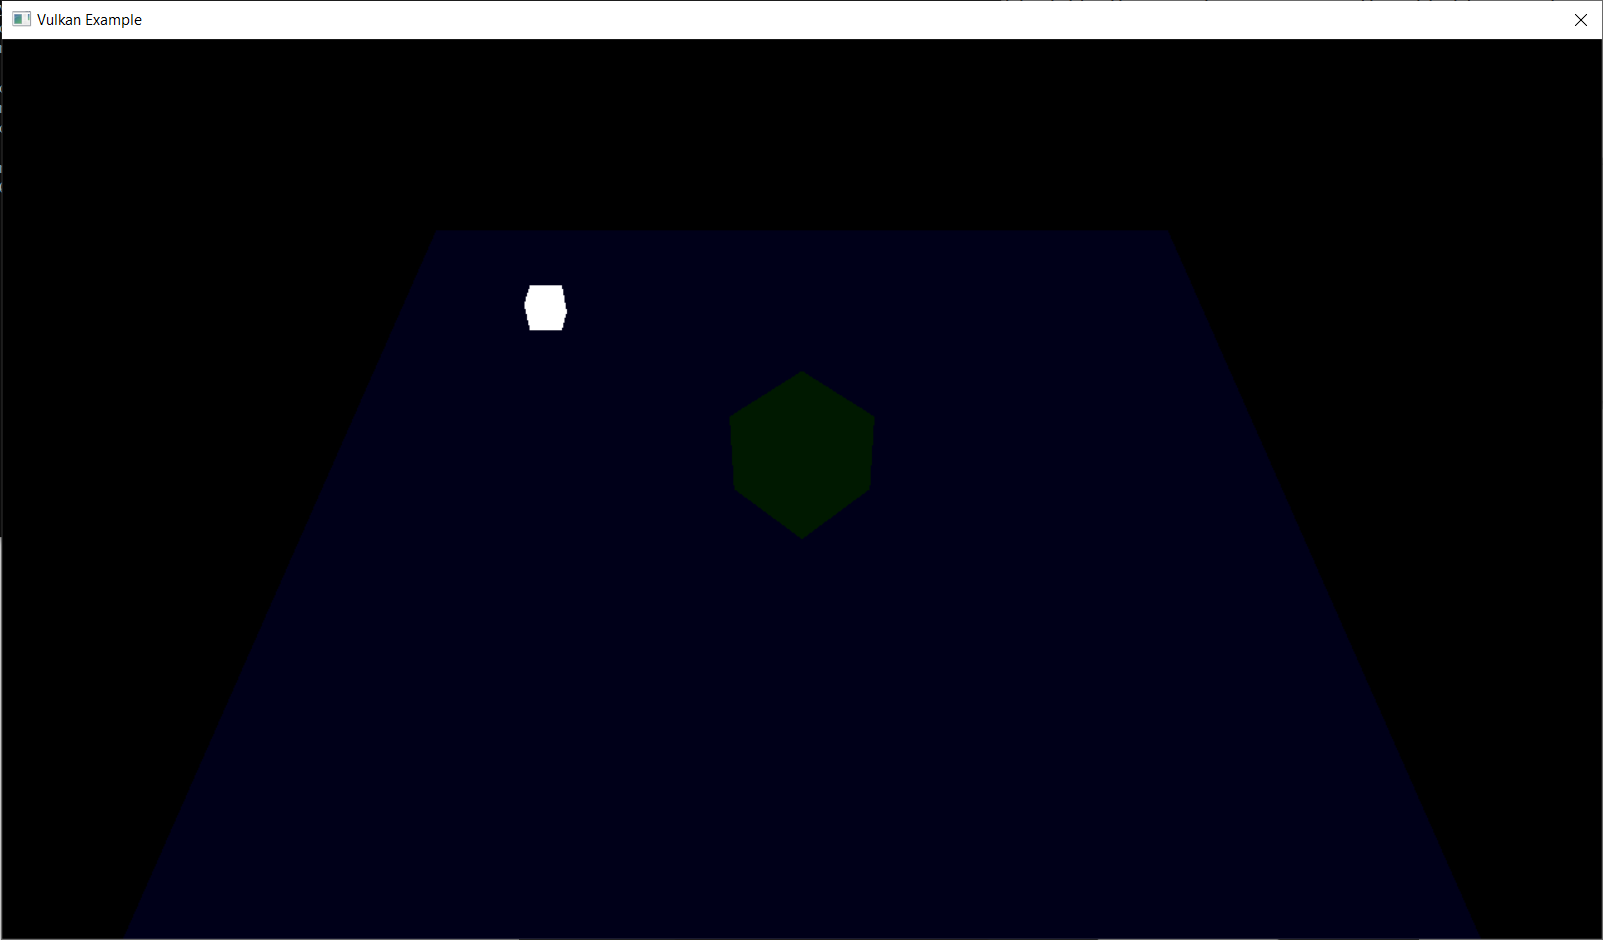
\includegraphics[scale=0.25]{images/ChBlinnPhong/SceneAmbient.png}
    \caption{Scene with ambient lighting}
    \label{fig::SceneAmbient}
\end{figure}

\section{Diffuse Lighting}

Diffuse lighting simulates the impact a light has on an object.
In simple terms, the more a part of the object faces the light, the brighter
it becomes.

Diffuse lighting gives the object more brightness the closer its fragments
are aligned to the light rays.

To compute the diffuse impact of the light on the fragment we take the dot
product between the surface's normal and the light direction.
The result is then multiplied with the light's color to get the diffuse component.
The greater the angle between the two vectors, the darker the diffuse component.

If the angle between the two vectors is greater than $90$ degrees, then the
diffuse impact will be negative.
We don't want this to happen.
Thus, all negative results will produce a zero diffuse impacts.

\begin{figure}[ht]
    \centering
    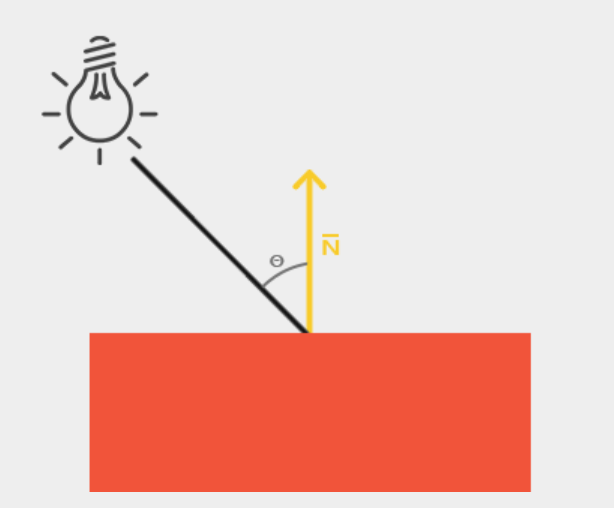
\includegraphics[scale=0.40]{images/ChBlinnPhong/DiffuseLighting.png}
    \caption{Computing diffuse lighting}
    \label{fig::ComputingDiffuseLighting}
\end{figure}

\begin{minipage}{\linewidth}{\noindent}
    \lstinputlisting[
        language=C++,
        caption={Computing diffuse component},
        label={lst::ShadeDiffuse}
        ]{src/ChBlinnPhong/ShadeDiffuse.frag}
\end{minipage}

\begin{figure}[ht]
    \centering
    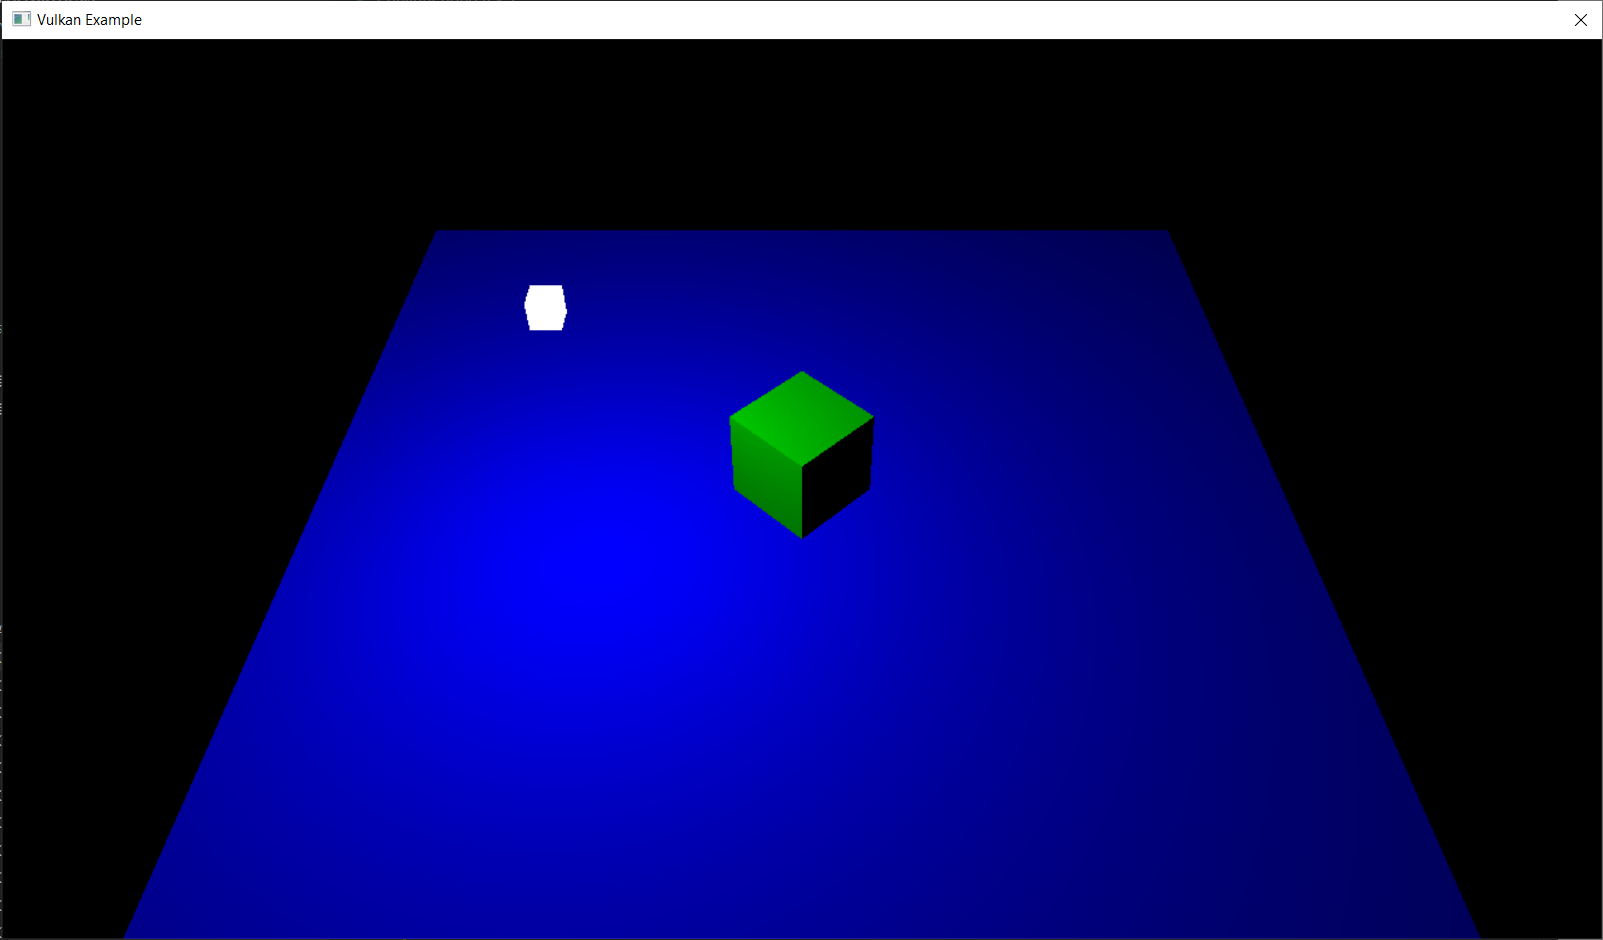
\includegraphics[scale=0.25]{images/ChBlinnPhong/SceneDiffuse.png}
    \caption{Scene with diffuse lighting}
    \label{fig::SceneDiffuse}
\end{figure}

\section{Specular Lighting}

Specular lighting simulates the bright spot that lights cause on bright objects.
This spot is called specular highlight.

\section{Materials}

\section{Light Properties}
